\section{Experimental Evaluation}
We evaluate DEFT in two settings: (i) a \emph{simulation analysis} and (ii) a \emph{real-world comparison}. We ask if a single policy can remain \emph{fail-active} under embodiment degradation. As shown in \cref{sec:sim-results}, \textsc{DEFT} consistently outperforms classical baselines on task success rate while under arbitrary, multi-joint failures and failures not seen during training. The real-world study further examines if these gains translate to end-to-end execution under induced multi-joint failures and primitive switches in real-world scenarios. Together, the results show that DEFT is a single policy that \emph{generalizes to arbitrary failure configurations}, \emph{completes multiple manipulation primitives}, and \emph{handles multi-joint failures}.
 \vspace{-5pt}

\subsection{Simulation Analysis} \label{sec:sim-analysis}
% We test three hypotheses: (\textbf{H.1}) DEFT increases \emph{constraint satisfaction} under joint-level failures compared to classical planners; (\textbf{H.2}) DEFT \emph{generalizes} to out-of-distribution (OOD) failures; and (\textbf{H.3}) DEFT maintains \emph{primitive-appropriate} motion (unconstrained and constrained) better than methods specialized to one primitive. \textbf{H.1} and \textbf{H.2} are designed to show DEFT's ability to generalize to arbitrary joint failures, and \textbf{H.3} is designed to show DEFT's ability to handle generate unconstrained and constrained primitive motions.
We test three hypotheses to probe DEFT’s generalization to arbitrary joint failures (\textbf{H1} and \textbf{H2}) and to test whether DEFT produces both unconstrained and constrained motions (\textbf{H3}).:

\begin{enumerate}[label=\textbf{H.\arabic*}]
\item Does DEFT obey embodiment constraints of arbitrary actuation failures more often than classical planners?
\item Does DEFT \emph{generalize} to out-of-distribution (OOD) failures?
\item Does DEFT adhere to constraint conditions more than approaches specialized to a single class of constraints?
\end{enumerate}



\subsubsection{Evaluation Preliminaries}\label{sec:eval-prelim}
Below, we define the task constraints geometrically, specify the dataset and baselines, and describe the in-domain (ID)–out-of-domain (OOD) partitioning in joint-limit space. Finally, we define the statistical procedures used to aggregate outcomes.


\paragraph{Evaluation Setup} 
We use the motion planning method from \cref{sec:data_generation} as our baseline, with RRT for \texttt{unconstrained} motions and differential IK with optimization for \texttt{constrained} motions. These baselines do not handle both primitives. In contrast, \textsc{DEFT} generates both within a unified model.

We evaluate on a fixed-base 7-dof Franka Emika Panda arm with the DEFT model inferencing on an NVIDIA RTX 4090. The study covers 4.7k failure conditions; of which 2.9k includes joint angle constraints (reduced and locked) and the rest are joint velocity constraints. For each condition, we randomly select 1–7 joints to be locked, range-limited, or velocity-restricted. Of these conditions, 22\% are in-domain (ID) and 78\% are out-of-domain (OOD). We classify ID/OOD using Mahalanobis (global) and k-NN (local) distances in joint space, labeling cases beyond the 95th percentile of either metric as OOD. Each unique failure condition is tested 100 times, each with 100 start-goal pairs for a total of 4.7M trajectories evaluated. Approximately 5\% of failure conditions render \texttt{constrained} motion infeasible and were excluded.

\begin{figure}
    \vspace{2mm}
    \centering
    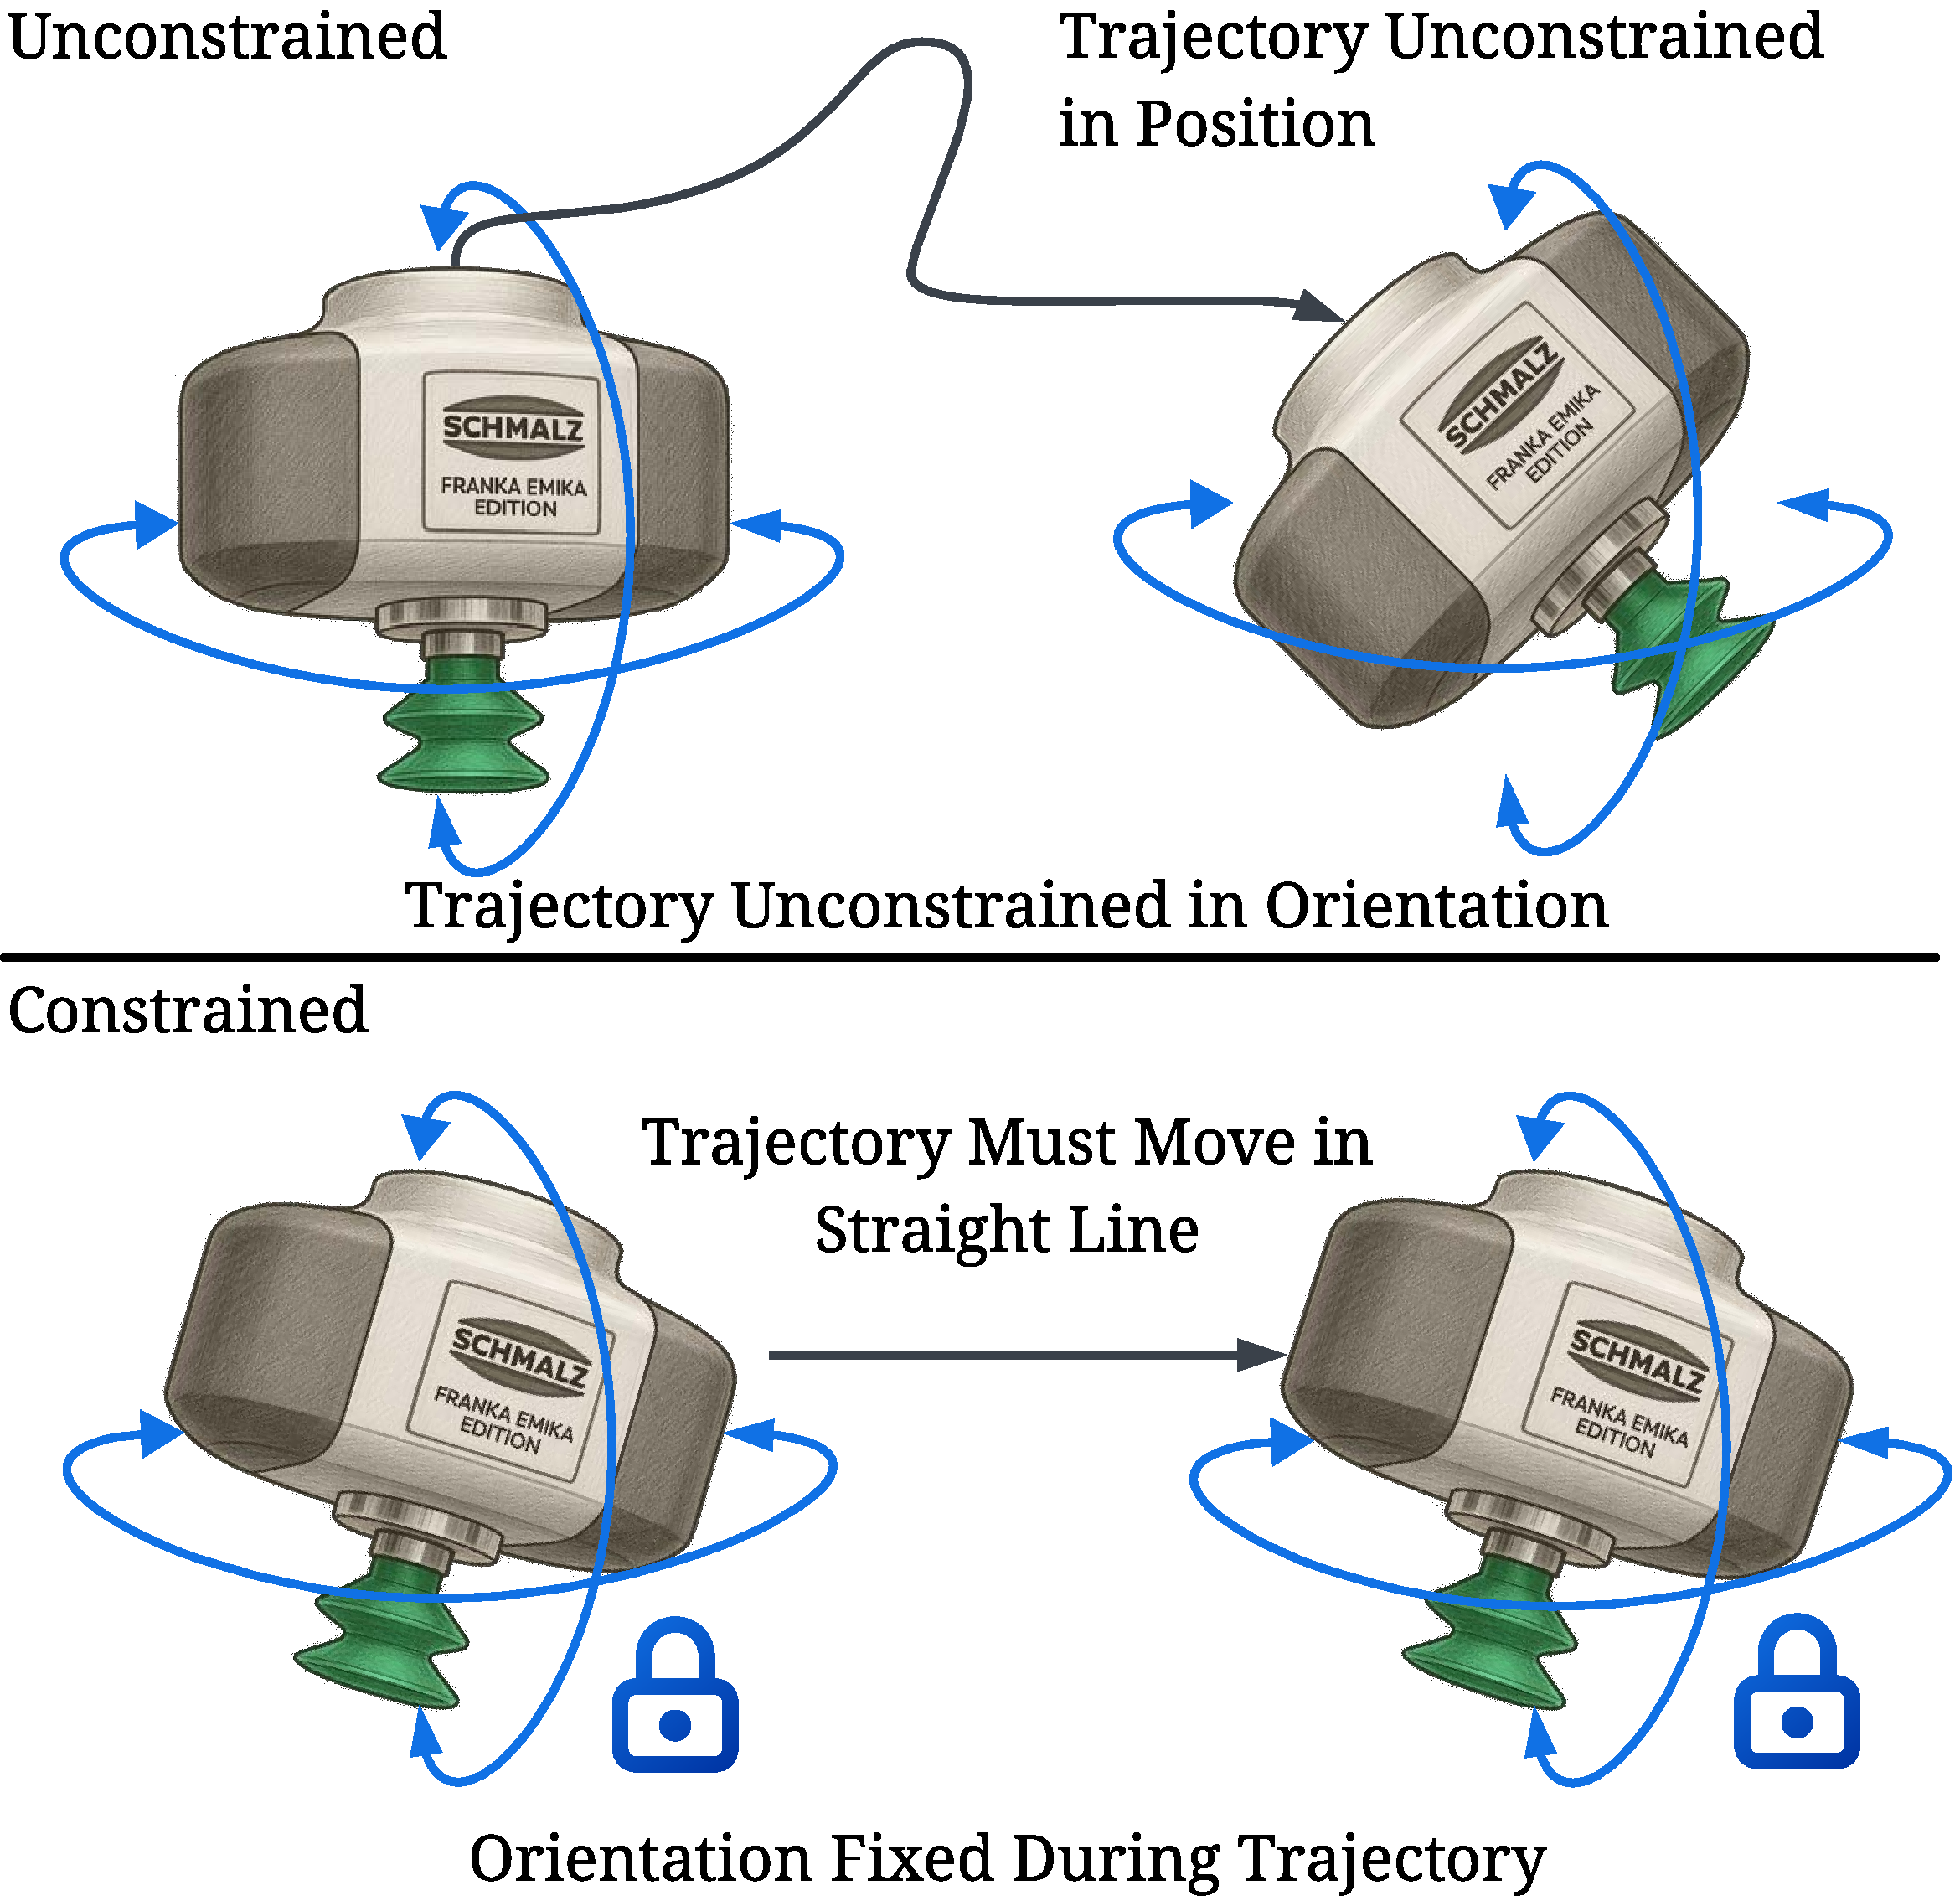
\includegraphics[width=0.9\columnwidth]{figures/primitives_explainer-compressed.pdf }
    \caption{Graphic description of the constraint definitions used in \cref{sec:sim-analysis}. The \texttt{unconstrained} primitive corresponds to a feasible trajectory between two points and includes unconstrained manipulation where the object is rigidly secured to the end-effector. The \texttt{constrained} corresponds to planar, approximately straight-line motion with minimal end-effector orientation change. \vspace{-25pt}}
    \label{fig:primitive-explain}
\end{figure}

\paragraph{Constraint Definitions}
Constraints correspond to task-relevant motion primitives. Unconstrained motion (\cref{fig:primitive-explain}, top) corresponds to a feasible trajectory between two points and includes manipulation primitives where the object is rigidly secured to the end-effector. The objective is to move from $\mathbf{q}_\text{s}\in\mathbb{R}^N$ to $\mathbf{q}_\text{g}\in\mathbb{R}^N$ with no additional geometric constraints beyond feasibility under failures.%
{\setlength{\abovedisplayskip}{6pt}\setlength{\belowdisplayskip}{6pt}\setlength{\abovedisplayshortskip}{4pt}\setlength{\belowdisplayshortskip}{4pt}%
\begin{equation}\small
\begin{aligned}
  \mathcal{T}_\text{Unconstrained}=\Big\{\mathbf{q}_t \forall t\in\{1,\dots,T\}\ \Big|\ 
  & \mathbf{q}_1=\mathbf{q}_\text{s},\  \mathbf{q}_T=\mathbf{q}_\text{g},\ \\
  & \mathbf{q}_t\in \mathcal{C}_t(\mathbf{q},\xi)\Big\}.
\end{aligned}
\end{equation}}%

Constrained motion (\cref{fig:primitive-explain}, bottom) corresponds to planar, approximately straight-line motion with minimal end-effector orientation change. This provides a spatial constraint for motion primitives such as pushing, pulling, or surface tracing. Let $\mathbf{p}_t\in\mathbb{R}^3$ be the end-effector position, $\mathbf{R}_t\in SO(3)$ its orientation, and $\mathbf{R}_\text{s}$ the initial orientation. Let $\mathcal{P}\subset\mathbb{R}^3$ be the designated plane. A trajectory satisfies \texttt{constrained} if, for all $t$, it obeys: (1) $\mathbf{p}_t\in\mathcal{P}$, (2) $\Delta p_t=\texttt{proj}_{\mathcal{P}}(\mathbf{p}_t)\le \epsilon_p$, (3) $\Delta \mathrm{R}_t=\|\mathbf{R}_t-\mathbf{R}_\text{s}\|_F\le \epsilon_R$, and (4) $\mathbf{q}_t\in \mathcal{C}_t(\xi)$. The valid trajectory set is:%
{\setlength{\abovedisplayskip}{6pt}\setlength{\belowdisplayskip}{6pt}\setlength{\abovedisplayshortskip}{4pt}\setlength{\belowdisplayshortskip}{4pt}%
\begin{equation}\small
\begin{aligned}
  \mathcal{T}_\text{Constrained}
  = \Big\{\mathbf{q}_{t}\ \forall t\in\{1,\dots,T\}\ \Big|\ &
  \mathbf{p}_t\in\mathcal{P}\ \land\ \\ \Delta p_t\le \epsilon_p,
   \Delta \mathrm{R}_t\le \epsilon_R\ & \land\ \mathbf{q}_t\in \mathcal{C}_t(\mathbf{q},\xi)
  \Big\}.
\end{aligned}
\end{equation}}%

\paragraph{Evaluation Metrics}
We applied statistical methods to test whether DEFT outperforms baseline approaches. Because success rates are bounded between 0 and 1 and often vary in spread, we used nonparametric methods that do not assume normally distributed data. To compare DEFT with the baseline under each failure condition, we estimated the difference in success rates using bootstrapping; if the 95\% confidence interval does not include zero, DEFT is considered better. To compare performance across groups of conditions (e.g., in-distribution vs. out-of-distribution, task constraint, or failure type), we used the Mann–Whitney U test, which is robust to unequal variances and outliers. To reduce the risk of false positives when making many comparisons, we applied false discovery rate (FDR) correction. Finally, to assess the overall effect of planner choice, we used a \(\chi^2\)\ test to ask whether using DEFT significantly changes the odds of satisfying constraints across all tasks.
%Together, these choices provide distribution-robust inference with controlled error rates that map directly to decisions an engineer would make (e.g., which planner to deploy).




% \begin{tabular}{|c|c|c|c|c|}
% \hline
% % \multicolumn{2}{|c|}{} & \multicolumn{3}{c|}{\textbf{Top Header for Last 3 Columns}} \\ \hline
% \multicolumn{2}{|c|}{} & \textbf{Baseline} & \textbf{DEFT} & \textbf{95\% C.I. } \\ \hline
% \multirow{H1} & Angle Failure & 48.2\% & \textbf{84.3}\% & [35.3\%-37.0\%]  \\ \cline{2-5}
%                          & Velocity Failure & 32.5\% & \textbf{70.8}\% & [37.8\%-38.8\%] \\ \hline
% \multirow{H2} & Constrained & 30.93\% & \textbf{46.42}\% & [--7.70\%, 34.50\%] \\ \cline{2-5}
%                          & Unconstrained & 42.4\% & \textbf{99.58\%} & [34.62\%, 79.85\%] \\ \hline
% \multirow{H3} & ID & \cellcolor{black} & \textbf{78.33\% }& \cellcolor{black} \\ \cline{2-5}
%                          & OOD & \cellcolor{black} & \textbf{73.61\%} & \cellcolor{black} \\ \hline
% \end{tabular}
% \caption{Success rate of the Baseline methods and the DEFT method. The 95\% Confidence Interval is on the improvement of DEFT over the baseline.}
% \label{tab:performance}
% \end{table}
% \vspace{5}
\subsubsection{Results} \label{sec:sim-results}
In this section, we demonstrate that DEFT significantly outperforms traditional planning baselines across various failure conditions. DEFT achieves a 37.66 percentage point improvement in constraint satisfaction compared to classical methods. We also show that DEFT generalizes well to unseen failure conditions, maintaining near-parity performance across in-distribution and out-of-distribution failure conditions. Finally, DEFT excels at handling both constrained and unconstrained motion tasks, with substantial gains in success rates across diverse constraints.
% We show within this setup, DEFT decisively outperforms classical baselines on all three hypotheses. \gm{add a teaser on what we show}



\paragraph{\textbf{H.1} Analysis}%
To evaluate whether DEFT produces trajectories that satisfy failure constraints at a higher rate than traditional planning baselines, we compare overall constraint satisfaction. DEFT achieves a success rate of 74.51\%, while the baseline achieves only 36.85\%. This represents an absolute improvement of 37.66 percentage points. A bootstrap analysis confirms the reliability of this difference ($p < 10^{-10}$), yielding a 95\% confidence interval of [37.21\%, 38.10\%] on the improvement in success rate. The specific performance rates for both angle and velocity failures can be seen in \cref{tab:performance}. Because the improvement holds across heterogeneous failure types and a wide range of sampled magnitudes, it indicates that DEFT generalizes to arbitrary joint-level degradations by conditioning directly on the failure embedding. In practice, given a new failure specification, DEFT translates it into feasible motion plans at substantially higher rates than the baseline.
 \vspace{-5pt}
% Further, we see significant improvments for angle and velocity failures for DEFT over the respective baselines, 84.3\% success rate for DEFT 48.2\% for the baseline in angle failure 
% The Mann-Whitney U with FDR correction for angle and velocity failures is  

\begin{table}[h]
\centering
\begin{tabular}{|c|c|c|c|}
\hline
\textbf{Hypothesis Summary} & \textbf{Test Condition}  & \textbf{Baseline} & \textbf{DEFT} \\ \hline
\textbf{H.1} Does DEFT handle & Angle Failure & 48.2\% & \textbf{84.3}\% \\ \cline{2-4}
arbitrary joint failures?& Velocity Failure & 32.5\% & \textbf{70.8}\% \\ \hline
\textbf{H.2} How well does DEFT & In Domain & \cellcolor{black} & \textbf{78.33\%} \\ \cline{2-4}
 handle unseen failures?& Out of Domain & \cellcolor{black} & \textbf{73.61\%} \\ \hline
\textbf{H.3} How well does DEFT  & Constrained & 30.93\% & \textbf{46.42}\% \\ \cline{2-4}
create multiple primitives?  & Unconstrained & 42.4\% & \textbf{99.58\%} \\ \hline

\end{tabular}
\caption{Success rate of the Baseline methods and the DEFT method. \vspace{-10pt}}
\label{tab:performance}
\end{table}

%   failure_type   deft_n  base_n  p_value  deft_success_rate  base_success_rate  significant  p_fdr
% 0        angle  1290400   13376      0.0           0.843308           0.482057         True    0.0
% 1     velocity  3417920   34822      0.0           0.707975           0.324852         True    0.0


\paragraph{\textbf{H.2} Analysis}
To test whether DEFT generalizes to unseen embodiment failure conditions, we tested success rates across in-distribution (ID) versus out-of-distribution (OOD) embodiment failure conditions, classified using Mahalanobis distance and k-NN distances in joint space. DEFT maintained a high constraint satisfaction rate as shown in \cref{tab:performance}. The small difference between ID and OOD performance indicates robustness to distributional shift. 
% In contrast, the baseline planner's OOD success rate was substantially lower (\textbf{37.70\%}).
Near-parity between ID and OOD success 
%, and the fact that even for failure conditions furthest from the training distribution (highest Mahalanobis-distance quartile) DEFT attains 68\% success,
indicates DEFT extrapolates over joint space rather than memorizing seen cases. Consequently, previously unseen failure configurations, regardless of which joint is affected or the magnitude of degradation, are translated into geometrically feasible, constraint-satisfying trajectories, evidencing DEFT’s ability to handle arbitrary failure conditions.



\paragraph{\textbf{H.3} Analysis}%
To assess whether DEFT more reliably satisfies task motion constraints, we evaluate performance separately for \texttt{unconstrained} (where the end effector can move freely, such as pick-and-place) and \texttt{constrained} (where the end effector must remain level and move in a straight line, such as surface tracing, pushing, and pulling) motions. The constraint satisfaction rate for both the categories as compared to the baselines (\cref{tab:performance}) shows that DEFT performs better for both primitives.
In the \texttt{unconstrained} setting, DEFT achieves a constraint satisfaction rate of 99.58\%, compared to 42.40\% for the RRT baseline, an absolute improvement of 57.18 percentage points. 
A Mann--Whitney U test on the \texttt{unconstrained} primitive difference between baseline and DEFT confirms that DEFT is statistically significant in 95.24\% of tested conditions after FDR correction, with a median bootstrap 95\% confidence interval on the improvement in success rate of [34.62\%, 79.85\%]. 
For the \texttt{constrained} motions, DEFT achieves 46.42\% satisfaction compared to the baseline's 30.93\%. A chi-squared test confirms that primitive constraint satisfaction is significantly associated with planner choice for both \texttt{unconstrained} and \texttt{constrained} primitives (\(\chi^2\text{ test},\ p<10^{-10}\)) , providing strong empirical support for \textbf{H.3}. It is important to note that the overall low success rate arises from the combined constraints of the primitive and the failure condition. For this evaluation, when excluding conditions, we checked only whether the randomly sampled start and goal satisfied the \texttt{constrained} constraints. However, this check does not guarantee that any feasible action exists, which likely contributes to the sub-50\% success rate.

These findings indicate that \textsc{DEFT} is not specialized to a single manipulation mode: it reliably synthesizes feasible trajectories for both \texttt{unconstrained} and \texttt{constrained} motions under the policy. 

\noindent\emph{Ablation note.} In simulation, conditioning yields similar constraint-obedience to an unconditioned diffusion ablation (within \(\approx\)1–2 percentage points overall), while delivering large gains in real-world task success (\cref{sec:real_world}).
 \vspace{-5pt}


\subsection{Real World}\label{sec:real_world}




Having established in simulation that \textsc{DEFT} generalizes to unseen failures and and reliably instantiates both \texttt{unconstrained} and \texttt{constrained} motions, we now test whether these gains translate to end-to-end task success on hardware. The next subsection evaluates \textsc{DEFT}, the hybrid RRT--Differential-IK optimization approach used in data generation (\cref{sec:data_generation}), and an ablation of DEFT without the conditioning input, \textsc{DEFT}-NoConditioning,  on two long-horizon, multi-primitive tasks (drawer and erasing). \vspace{-15pt}

% \begin{table}[h]
% \centering
% \caption{Drawer configuration: applied joint limits (rad).}
% \label{tab:limits_drawer}
% \setlength{\tabcolsep}{5pt}\footnotesize
% \begin{tabular}{lrrl}
% \hline
% \textbf{Joint} & \textbf{Lower} & \textbf{Upper} & \textbf{Note} \\
% \hline
% $J_1$ & 0.049775 & 0.049775 & LOCKED \\
% $J_2$ & -1.762800 & 1.762800 & NORMAL \\
% $J_3$ & -2.897300 & 2.897300 & NORMAL \\
% $J_4$ & -2.470927 & -1.925254 & REDUCED \\
% $J_5$ & -2.897300 & 2.897300 & NORMAL \\
% $J_6$ & 1.195150 & 2.623850 & REDUCED \\
% $J_7$ & -2.897300 & 2.897300 & NORMAL \\
% \hline
% \end{tabular}
% \end{table}

% \begin{table}[h]
% \centering
% \caption{Eraser (Whiteboard) configuration: applied joint limits (rad).}
% \label{tab:limits_eraser}
% \setlength{\tabcolsep}{5pt}\footnotesize
% \begin{tabular}{lrrl}
% \hline
% \textbf{Joint} & \textbf{Lower} & \textbf{Upper} & \textbf{Note} \\
% \hline
% $J_1$ & 0.033067 & 1.027757 & REDUCED \\
% $J_2$ & -1.762800 & 1.762800 & NORMAL \\
% $J_3$ & -2.897300 & 2.897300 & NORMAL \\
% $J_4$ & -3.071800 & -0.069800 & NORMAL \\
% $J_5$ & -0.073072 & 0.956709 & REDUCED \\
% $J_6$ & 1.865146 & 2.958065 & REDUCED \\
% $J_7$ & -2.897300 & 2.897300 & NORMAL \\
% \hline
% \end{tabular}
% \end{table}

\begin{table}[h]
\centering
\caption{Applied joint limits (rad) for real-world configurations. \textbf{Bold} indicates a locked joint; \emph{italics} indicate reduced limits.}
\label{tab:limits_drawer_eraser}
\setlength{\tabcolsep}{6pt}\footnotesize
\begin{tabular}{lrr|rr}
\hline
\textbf{Joint} & \multicolumn{2}{c|}{\textbf{Drawer}} & \multicolumn{2}{c}{\textbf{Erasing}} \\
 & \textbf{Lower} & \textbf{Upper} & \textbf{Lower} & \textbf{Upper} \\
\hline
$J_1$ & \emph{-0.81} & \emph{0.17} & \emph{0.033} & \emph{1.028} \\
$J_2$ & \emph{0.10} & \emph{1.50} & -1.763 & 1.763 \\
$J_3$ & \emph{-0.90} & \emph{0.60} & -2.897 & 2.897 \\
$J_4$ & \emph{-2.60} & \emph{-1.30} & \textbf{-2.59} & \textbf{-2.59}\\
$J_5$ & \emph{-0.10} & \emph{1.70} & \emph{-0.073} & \emph{0.957} \\
$J_6$ & \emph{0.90} & \emph{2.50} & \emph{1.865} & \emph{2.958} \\
$J_7$ & \emph{-0.85} & \emph{1.60} & -2.897 & 2.897 \\
\hline
\end{tabular}
\end{table}
\vspace{-10pt}

\begin{figure}[hbtp]
\vspace{2mm}
  \centering
  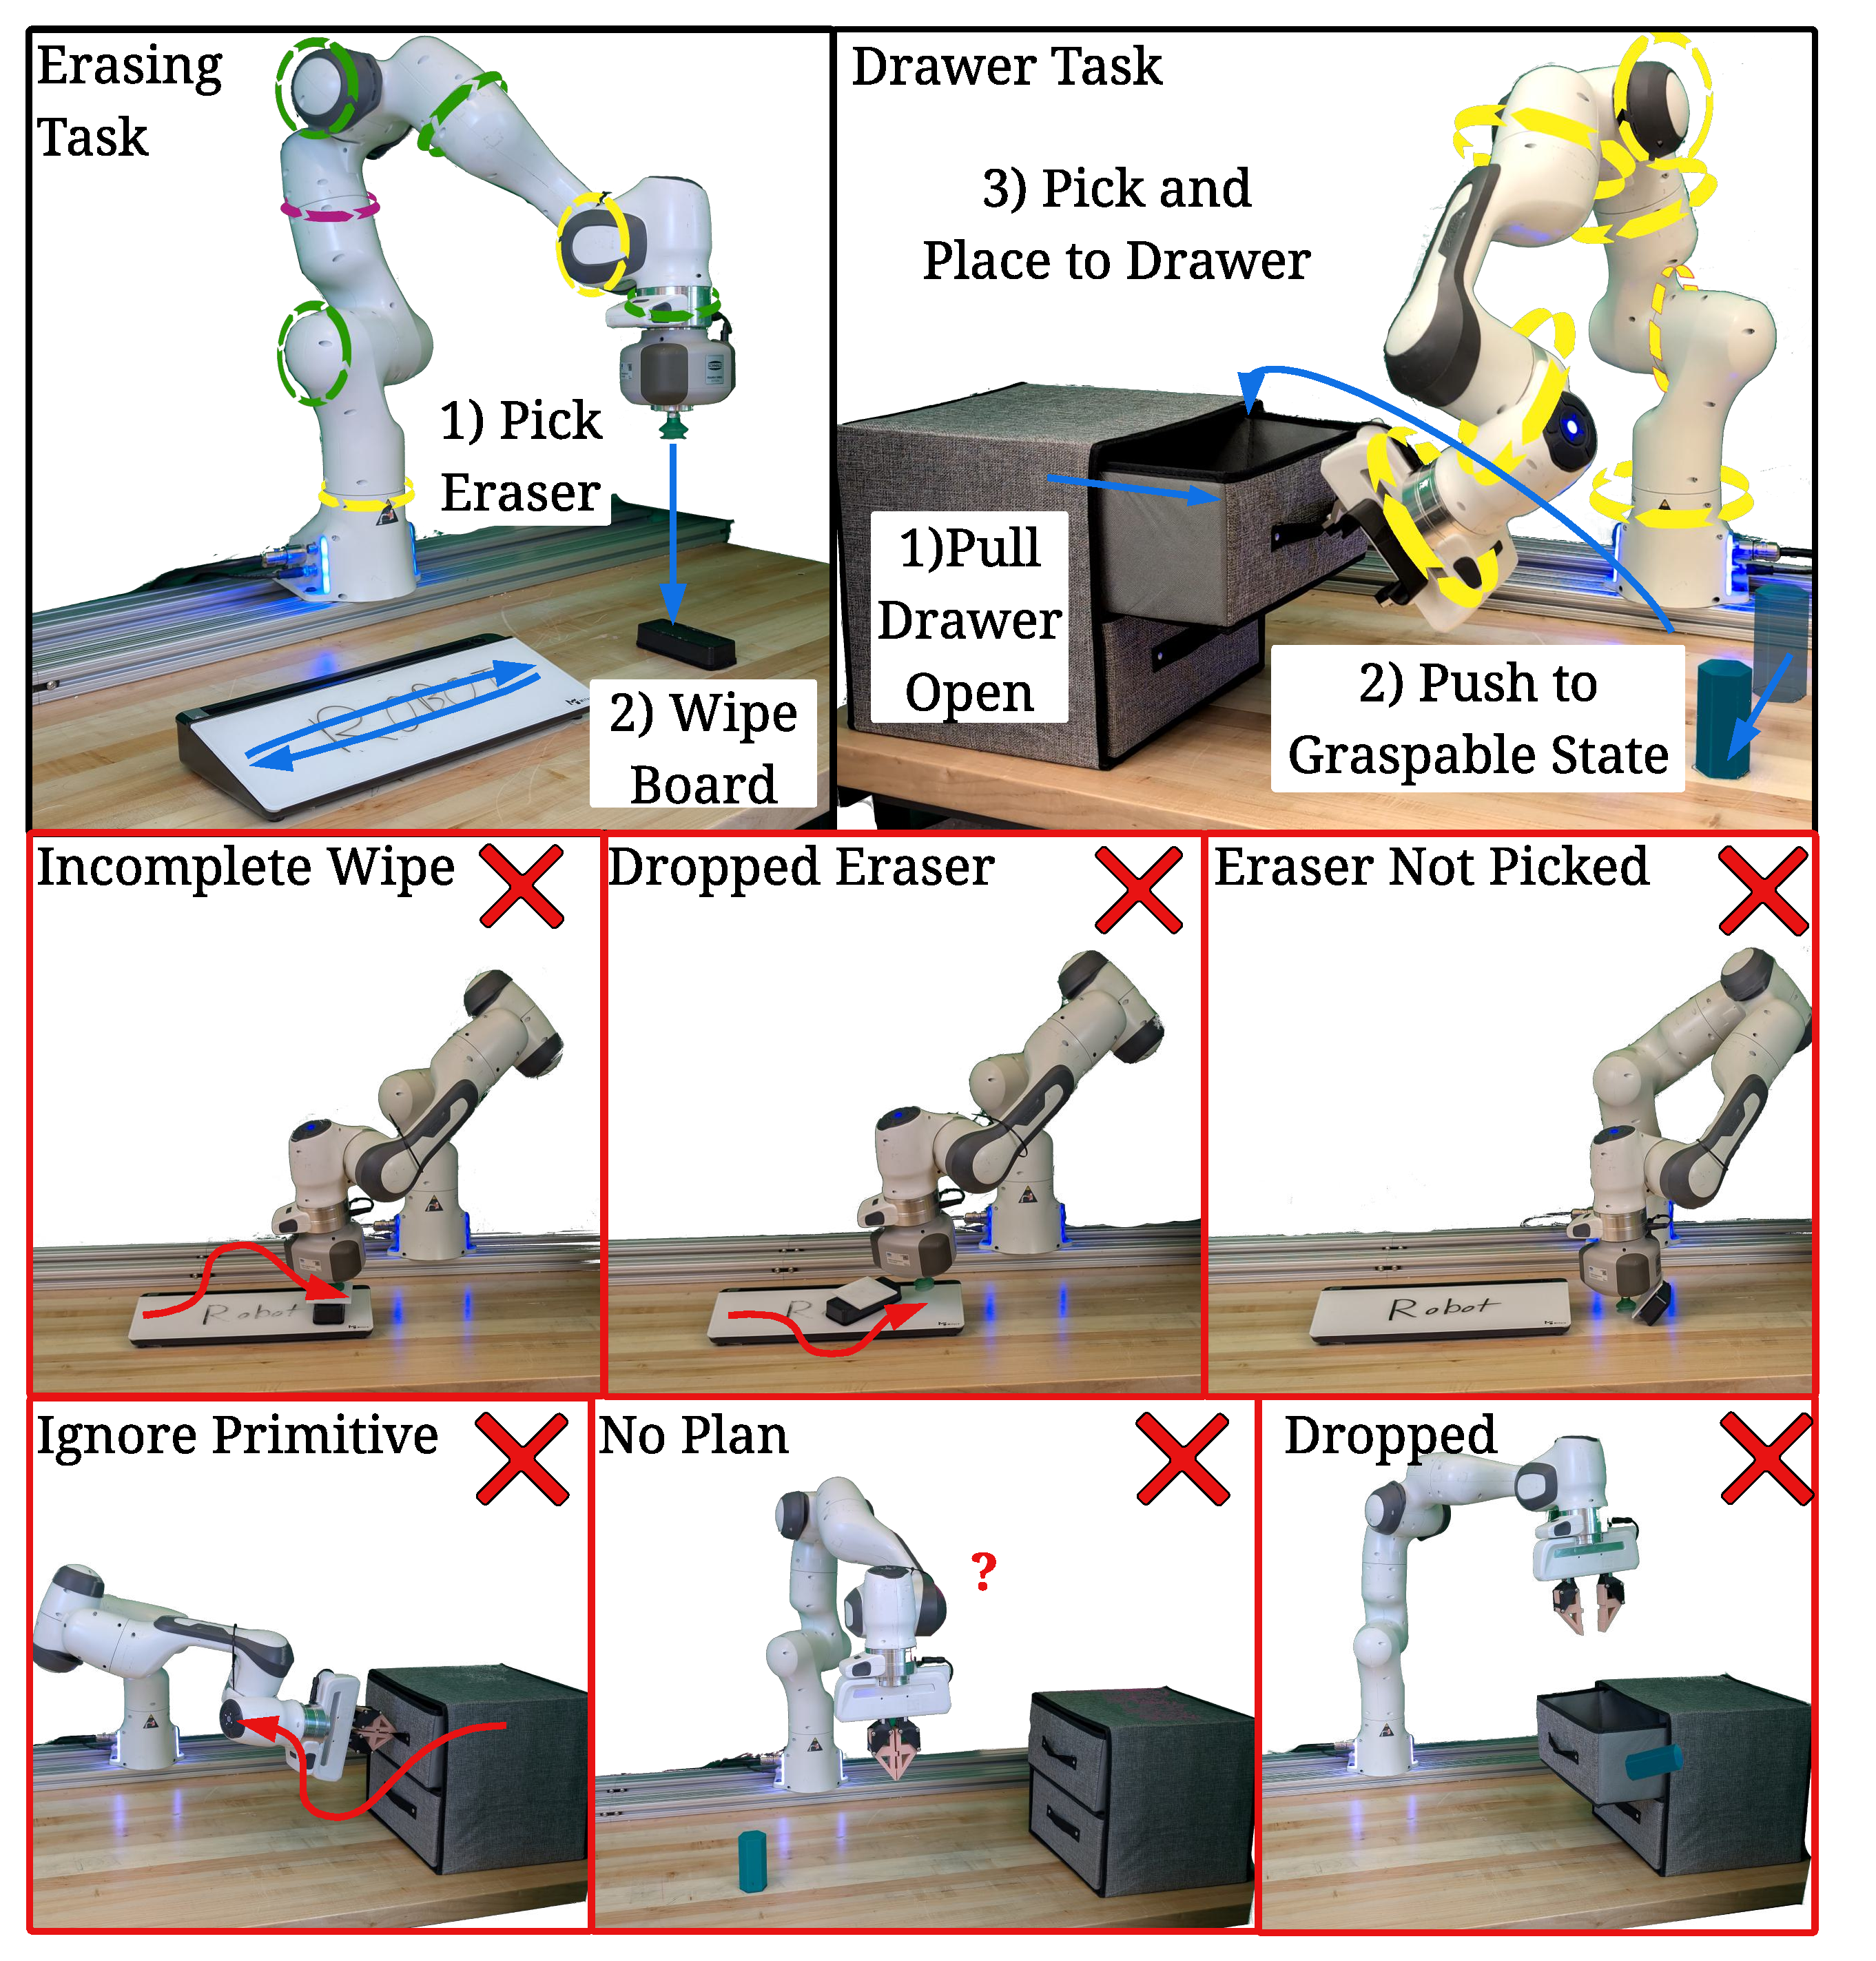
\includegraphics[width=\columnwidth]{figures/real-task-explainer-vertical-compressed-1.pdf}

  \caption{Left (Erasing): The robot grasps an eraser from the table and performs back-and-forth sweeps to remove text. Erasing failures include incomplete wipes or drops from disobeying motion constraints (improper normal force), and missed picks when lacking inpainting prevents reaching prescribed start/goal poses. Right (Drawer): The robot opens a drawer, pushes an object to a graspable pose, places it inside, and closes the drawer. Drawer failures include unopened drawers from ignored motion constraints, unfeasible plans under task constraints, and drops from unrespected target positions without inpainting.\vspace{-23pt}}
  \label{fig:real-world-tasks}
\end{figure}


\subsubsection{Task Description}  
We evaluate our system on two long-horizon, multi-step manipulation tasks that integrate both unconstrained and constrained actions, and that require transitions between unconstrained free-space motion and constrained contact-rich interaction. 

\paragraph{Drawer Task} (\cref{fig:real-world-tasks}, Top Right)
The drawer task consists of five sequential phases: (1) pulling the drawer open from its closed state, (2) pushing the object to a graspable position, (3) grasping an object from the workspace, (4) placing the object inside the drawer, and (5) pushing the drawer closed. The task combines unconstrained manipulation (picking and placing) with constrained manipulation (pushing and pulling), while alternating between unconstrained free-space motion and the constrained kinematics of the drawer. This structure creates distinct primitive requirements and embodiment sensitivities, making it effective for evaluating how conditioning and inpainting influence robustness. 

We assign scores of 1.0 for completing the task and 0.0 for not completing the task as all observed errors led to complete task failure. We evaluated 10 runs per approach.

\paragraph{Erasing Task}  
The erasing task requires the robot to first grasp an eraser from the table, then sweep it back and forth across a whiteboard to remove pre-written text. Here, unconstrained manipulation (picking) leads into constrained, contact-rich surface motion (erasing), requiring sustained alignment with the constrained geometry of the board. This task emphasizes embodiment-dependent failure recovery in a setting where continuous constraint satisfaction and primitive-specific control are necessary, providing a complementary evaluation to the drawer task. 

We partially score each trial up to 1.0 point: (i) +0.25 for picking the eraser, (ii) +0.50 for removing the target text with points awarded only for full removal of markings on the board, and (iii) +0.25 for retaining the eraser through the run. We evaluated 10 runs per approach.

\subsubsection{Failure Condition Description}
% For reproducibility, we list the joint limits enforced on the physical robot in \cref{tab:limits_drawer_eraser}. In the drawer task (\cref{fig:real-world-tasks}, right), locking $J_1$ removes base yaw, reducing the arm from seven to six degrees of freedom and eliminating a major redundancy axis. Narrowing the ranges of $J_4$ and $J_6$ restricts elbow and wrist motion, shrinking both the reachable and orientation workspaces, reducing null-space freedom, and lowering manipulability. In the erasing task (\cref{fig:real-world-tasks}, left), tightening $J_1$, $J_5$, and $J_6$ further limits global heading changes and wrist flexion/rotation, making orientation-constrained motions harder to realize.
For reproducibility, we list the joint limits enforced on the physical robot in \cref{tab:limits_drawer_eraser}. In the drawer task, all seven joints operate under reduced ranges. Collectively, these reductions shrink both reachable and orientation workspaces, diminish null-space freedom, and lower manipulability. In the erasing task, the elbow $J_4$ is locked at $-2.4$\,rad, removing one degree of freedom; $J_1$, $J_5$, and $J_6$ are reduced, further constraining end effector rotation and positioning.


\subsubsection{Results}
In the following section, we present real-world task results that further validate the findings from our simulations. \textsc{DEFT} consistently outperforms traditional baselines, achieving perfect task completion in both the Drawer and Erasing tasks. These results underscore the robustness of \textsc{DEFT} in handling joint-limit failures, showing how embodiment and primitive conditioning enable stable, feasible motion plans where optimization-based methods fail.
\vspace{-15pt}
\begin{table}[h]
\centering
\caption{Real-world task results over 10 runs. }
\label{tab:rw_tasks_combined}
\begingroup
\setlength{\tabcolsep}{5pt}
\renewcommand{\arraystretch}{1.1}
\footnotesize
\begin{tabular}{@{}llcc@{}}
\hline
\textbf{Model} & \textbf{Task} & \textbf{Mean} & \textbf{Std.}  \\
\hline
DEFT                & Drawer  & \textbf{1.00} & 0.00  \\
DEFT                & Erasing & \textbf{1.00} & 0.00 \\
Optimization        & Drawer  & 0.00 & 0.00 \\
Optimization        & Erasing & 0.35 & 0.32 \\
DEFT-NoConditioning & Drawer  & 0.60 & 0.49 \\
DEFT-NoConditioning & Erasing & 0.93 & 0.12 \\
\hline
\end{tabular}
\endgroup
\end{table}
\vspace{-11pt}
\paragraph{Drawer Task}
\textsc{DEFT} achieved perfect task completion on the drawer task (\cref{tab:rw_tasks_combined}). The Optimization baseline produced no executable plans. \textsc{DEFT}-NoConditioning succeeded in \(6/10\) runs. Qualitatively, Optimization repeatedly failed to find feasible trajectories in the constrained drawer setting. The unconditioned ablation failed for two reasons: 1) the lack of embodiment conditioning and 2) missing start--goal inpainting. These missing components caused surface-constraint violations and jerky motion leading to the robot dropping the object and being unable to open the drawer. \textsc{DEFT} alternated cleanly between unconstrained pick-and-place and constrained push and pulls without violating joint or contact limits.

\paragraph{Erasing Task}
\textsc{DEFT} again achieved perfect completion (\cref{tab:rw_tasks_combined}). The Optimization baseline had a success rate of 35\% and exhibited unstable surface interaction with poor contact maintenance. \textsc{DEFT}-NoConditioning had a success rate of 93\% but would disobey the contact constraints causing the robot to lose control of the eraser, consistent with missing embodiment conditioning and inpainting. Under a severe configuration (elbow locked at \(J_4=-2.4\,\mathrm{rad}\) with reduced wrist and base limits), \textsc{DEFT} maintained smooth, constraint-consistent sweeps while preserving grasp.

These outcomes support our central hypothesis: embodiment and task conditioning, coupled with inpainting and clamping, yield a policy that remains fail-active under embodiment degradation. 
Practically, they show that \textsc{DEFT} recovers performance in settings where traditional optimization either cannot plan or produces unstable motions, and where an unconditioned generative policy is brittle. 
Together with the simulation results, the real-world trials substantiate that a single conditioned diffusion policy sustains task success across multiple primitives and joint-limit failures. 
%Overall, we show that \textsc{DEFT} preserves functionality across failures through completing tasks that require continuous constraint satisfaction and behavior switching.


 % Across both tasks, \textsc{DEFT}’s embodiment- and primitive-aware conditioning (with joint-limit inpainting) yields reliable, constraint-compliant behavior: it achieves perfect completion and adherence to the intended motion primitive on every run. The optimization baseline struggles to discover robust contact sequences: in drawer closing it only achieved closure once (and did not reach perfect compliance), and in erasing it produced erratic, unstable contact with just one full success. The unconditioned diffusion policy (DEFT-NoConditioning) demonstrates strong task completion but systematically ignores the NPM constraint—scoring 0.75 on every drawer run and frequently dropping performance during contact-rich wiping—highlighting that conditioning and inpainting are not cosmetic, but necessary to enforce primitives and sustain reliable contact over long horizons. 


